% Options for packages loaded elsewhere
\PassOptionsToPackage{unicode}{hyperref}
\PassOptionsToPackage{hyphens}{url}
%
\documentclass[
]{article}
\usepackage{amsmath,amssymb}
\usepackage{iftex}
\ifPDFTeX
  \usepackage[T1]{fontenc}
  \usepackage[utf8]{inputenc}
  \usepackage{textcomp} % provide euro and other symbols
\else % if luatex or xetex
  \usepackage{unicode-math} % this also loads fontspec
  \defaultfontfeatures{Scale=MatchLowercase}
  \defaultfontfeatures[\rmfamily]{Ligatures=TeX,Scale=1}
\fi
\usepackage{lmodern}
\ifPDFTeX\else
  % xetex/luatex font selection
\fi
% Use upquote if available, for straight quotes in verbatim environments
\IfFileExists{upquote.sty}{\usepackage{upquote}}{}
\IfFileExists{microtype.sty}{% use microtype if available
  \usepackage[]{microtype}
  \UseMicrotypeSet[protrusion]{basicmath} % disable protrusion for tt fonts
}{}
\makeatletter
\@ifundefined{KOMAClassName}{% if non-KOMA class
  \IfFileExists{parskip.sty}{%
    \usepackage{parskip}
  }{% else
    \setlength{\parindent}{0pt}
    \setlength{\parskip}{6pt plus 2pt minus 1pt}}
}{% if KOMA class
  \KOMAoptions{parskip=half}}
\makeatother
\usepackage{xcolor}
\usepackage[margin=1in]{geometry}
\usepackage{graphicx}
\makeatletter
\def\maxwidth{\ifdim\Gin@nat@width>\linewidth\linewidth\else\Gin@nat@width\fi}
\def\maxheight{\ifdim\Gin@nat@height>\textheight\textheight\else\Gin@nat@height\fi}
\makeatother
% Scale images if necessary, so that they will not overflow the page
% margins by default, and it is still possible to overwrite the defaults
% using explicit options in \includegraphics[width, height, ...]{}
\setkeys{Gin}{width=\maxwidth,height=\maxheight,keepaspectratio}
% Set default figure placement to htbp
\makeatletter
\def\fps@figure{htbp}
\makeatother
\setlength{\emergencystretch}{3em} % prevent overfull lines
\providecommand{\tightlist}{%
  \setlength{\itemsep}{0pt}\setlength{\parskip}{0pt}}
\setcounter{secnumdepth}{-\maxdimen} % remove section numbering
\usepackage{amsmath}
\ifLuaTeX
  \usepackage{selnolig}  % disable illegal ligatures
\fi
\usepackage{bookmark}
\IfFileExists{xurl.sty}{\usepackage{xurl}}{} % add URL line breaks if available
\urlstyle{same}
\hypersetup{
  pdftitle={Assignment 1},
  pdfauthor={Jakob og Oskar},
  hidelinks,
  pdfcreator={LaTeX via pandoc}}

\title{Assignment 1}
\author{Jakob og Oskar}
\date{2025}

\begin{document}
\maketitle

\section{Assignment 1 in interpretable machine
learning}\label{assignment-1-in-interpretable-machine-learning}

We are tasked with building a predictive regression model, with the best
possible prediction. This submission will be split up into several
parts:

\begin{itemize}
\tightlist
\item
  Initial data preprocessing and overview
\item
  Introduction into the mathematics
\item
  Modelling and justification
\item
  Comparative discussion
\end{itemize}

\subsection{Initial data preprocessing and
overview}\label{initial-data-preprocessing-and-overview}

The given data has the form:

\begin{verbatim}
##  [1] "ID"                   "Date_start_contract"  "Date_last_renewal"   
##  [4] "Date_next_renewal"    "Date_birth"           "Date_driving_licence"
##  [7] "Distribution_channel" "Seniority"            "Policies_in_force"   
## [10] "Max_policies"         "Max_products"         "Lapse"               
## [13] "Date_lapse"           "Payment"              "Premium"             
## [16] "Cost_claims_year"     "N_claims_year"        "N_claims_history"    
## [19] "R_Claims_history"     "Type_risk"            "Area"                
## [22] "Second_driver"        "Year_matriculation"   "Power"               
## [25] "Cylinder_capacity"    "Value_vehicle"        "N_doors"             
## [28] "Type_fuel"            "Length"               "Weight"
\end{verbatim}

We are asked to predict the \textbf{Cost\_claims\_year} given the rest
of the covariate-vector. Initially it is important to note that out data
is a classical insurance dataset, where we are given rows corresponding
to insurance periode for a given contract. There are several issues with
this, since some contracts might overlap into multiple contracts, which
can be identified by the ID. It is however very difficult to locate
these policies, and we overlook this issue.

There are numerous char. vectors in the data, which can be seen here:

\begin{verbatim}
## Classes 'data.table' and 'data.frame':   105555 obs. of  30 variables:
##  $ ID                  : int  1 1 1 1 2 2 3 3 3 3 ...
##  $ Date_start_contract : chr  "05/11/2015" "05/11/2015" "05/11/2015" "05/11/2015" ...
##  $ Date_last_renewal   : chr  "05/11/2015" "05/11/2016" "05/11/2017" "05/11/2018" ...
##  $ Date_next_renewal   : chr  "05/11/2016" "05/11/2017" "05/11/2018" "05/11/2019" ...
##  $ Date_birth          : chr  "15/04/1956" "15/04/1956" "15/04/1956" "15/04/1956" ...
##  $ Date_driving_licence: chr  "20/03/1976" "20/03/1976" "20/03/1976" "20/03/1976" ...
##  $ Distribution_channel: chr  "0" "0" "0" "0" ...
##  $ Seniority           : int  4 4 4 4 4 4 15 15 15 15 ...
##  $ Policies_in_force   : int  1 1 2 2 2 2 1 1 1 1 ...
##  $ Max_policies        : int  2 2 2 2 2 2 2 2 2 2 ...
##  $ Max_products        : int  1 1 1 1 1 1 1 1 1 1 ...
##  $ Lapse               : int  0 0 0 0 0 0 0 0 0 0 ...
##  $ Date_lapse          : chr  "" "" "" "" ...
##  $ Payment             : int  0 0 0 0 1 1 0 0 0 0 ...
##  $ Premium             : num  223 214 215 217 214 ...
##  $ Cost_claims_year    : num  0 0 0 0 0 0 0 0 0 0 ...
##  $ N_claims_year       : int  0 0 0 0 0 0 0 0 0 0 ...
##  $ N_claims_history    : int  0 0 0 0 0 0 0 0 0 0 ...
##  $ R_Claims_history    : num  0 0 0 0 0 0 0 0 0 0 ...
##  $ Type_risk           : int  1 1 1 1 1 1 3 3 3 3 ...
##  $ Area                : int  0 0 0 0 0 0 0 0 0 0 ...
##  $ Second_driver       : int  0 0 0 0 0 0 0 0 0 0 ...
##  $ Year_matriculation  : int  2004 2004 2004 2004 2004 2004 2013 2013 2013 2013 ...
##  $ Power               : int  80 80 80 80 80 80 85 85 85 85 ...
##  $ Cylinder_capacity   : int  599 599 599 599 599 599 1229 1229 1229 1229 ...
##  $ Value_vehicle       : num  7068 7068 7068 7068 7068 ...
##  $ N_doors             : int  0 0 0 0 0 0 5 5 5 5 ...
##  $ Type_fuel           : chr  "P" "P" "P" "P" ...
##  $ Length              : num  NA NA NA NA NA ...
##  $ Weight              : int  190 190 190 190 190 190 1105 1105 1105 1105 ...
##  - attr(*, ".internal.selfref")=<externalptr> 
## NULL
\end{verbatim}

One could, model some of the char. vectors like proposed in the
lectures, by

\begin{align*}
 X_i &= E(Y \mid X_i ) \\
 &=\int_Y y\ \mu(x, dy)
\end{align*}

where \(\mu\) is the appropriate probability kernel, and we let \(y\) be
our response. However, we choose to take the our char. vectors and round
them to yearly values, which then has a ordinal ordering and can thus be
used as features. Further we take and one-hot encode
\emph{Distribution\_channel} by creating three new features which are
either \(1\) or \(0\). Same for the type of fuel.

Next there are some missing values.

\begin{figure}

{\centering 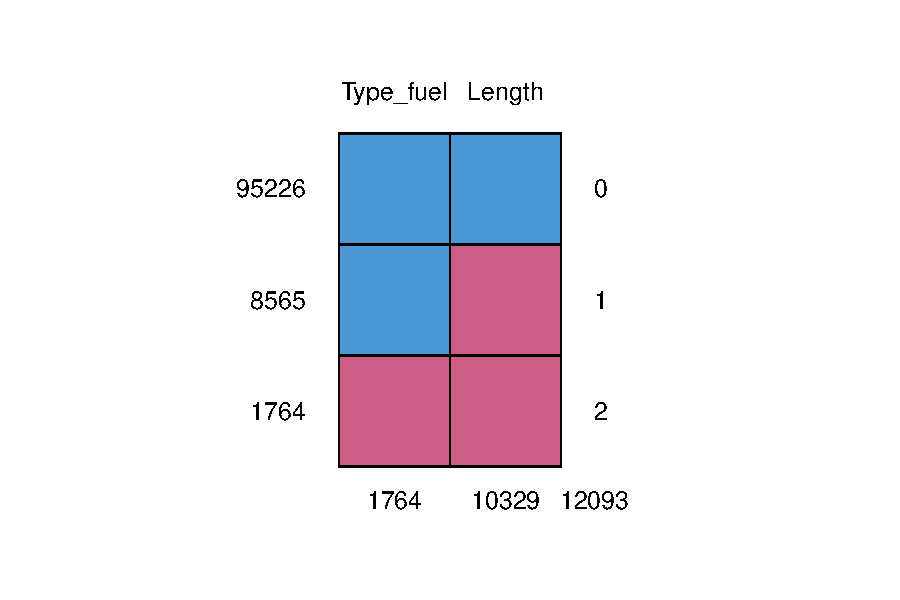
\includegraphics[width=0.5\linewidth]{assignment_uptodat_files/figure-latex/unnamed-chunk-6-1} 

}

\caption{Missing data plot, right axis shows numer of missing columns in that row, and the left axis show how many rows have this missingness pattern}\label{fig:unnamed-chunk-6}
\end{figure}

\begin{verbatim}
##       Type_fuel Length      
## 95226         1      1     0
## 8565          1      0     1
## 1764          0      0     2
##            1764  10329 12093
\end{verbatim}

It becomes apparent that there are missing values in the length and
type\_fuel variable. We can see that the missingness is overlapping in
\(1764\) rows. However the length variable suffers way heavier from
missingnes compared to type\_fuel. In order to impute values, we assume
the missingnes it completely at random for both features. We consider
correlated features to do imputation. We see from the correlation plot
(fig. @ref(fig:corplot)) that type\_fuel is mostly correlated with
Cylinder\_capacity, Value\_vehicle and Weight. The same goes for the
feature Length. Therefore, we fit a multivariate linear regression model
with these 3 covariates to predict both type\_fuel and Length (using
cbind in the response formula). Finally, we predict the missing values
using this trained model

Finally we look at the correlation between the covariates.

\begin{figure}

{\centering 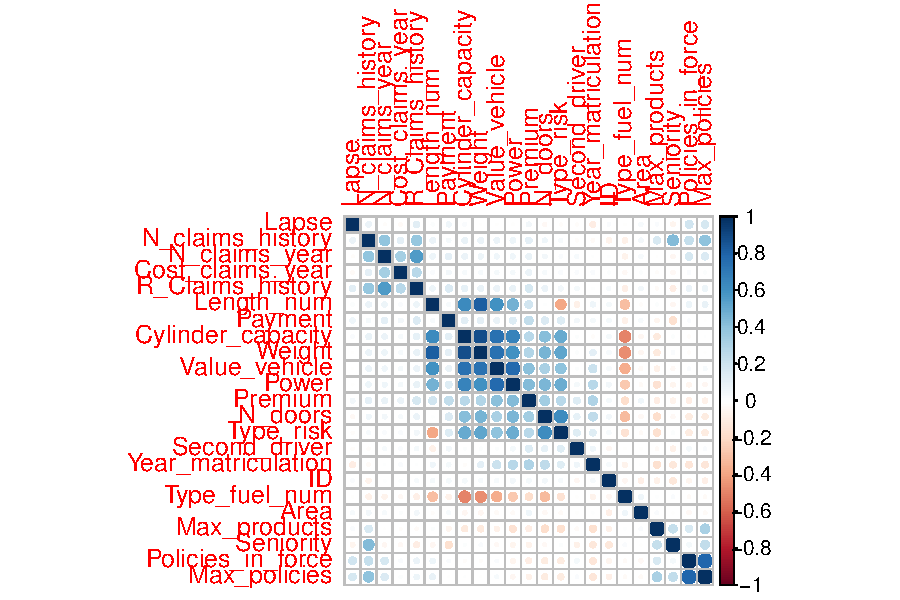
\includegraphics{assignment_uptodat_files/figure-latex/corplot-1} 

}

\caption{Correlation plot between the continious covariates}\label{fig:corplot}
\end{figure}

We notice some clusters, most meaningfull between
\emph{Cylinder\_capacity}, \emph{Value\_vehicle} and \emph{Weight} which
is expected. We deem these to have significant predictive ability, and
thus we choose to not remove these. The top left cluster, will be
ignored for now, since we will later introduce a data-transformation
which affects this cluster in a high degree.

\subparagraph{Data Aggregation}\label{data-aggregation}

For our data aggregation we want to have the ability to assume
independence, which we have if we aggregate the rows into being one
policy. There are several problems to tacle to achive data in the
desired format. We have to both choose an appropriate aggreations
function, and we have to consider events where the insured object
change. We start off by identifying some unique-identifiers. If theme
columns change, we deem the contract to insure a new car, or at least
insure something that is independent of what was previously insured.
Amongst these unique identifiers are Length, Weight, Power etc. so
things which change, probably mean that the thing that is insured has
changes. \textbackslash{} Next, we look at how we have aggregated data.
Firstly we sum the exposure for each contract, since we will use this to
weight in the models later on. Next we use the max function on the
number of policies, lapse, date of birth, date of driving licence, start
of contract, products, payments, ratio of claims history, type of risk,.
For The mean premium we use the mean of the premium without the forward
premium, that is the premium for the time we want to predict for. For
the value of the veichle, and number of doors we use mean. For the
length we use sum since this is just a scaling. For the variable
\emph{cost\_claims\_this\_year} we use the cost of the claims in
\(\mathcal{F}_t\) where we are to predict data on \(\mathcal{F}_{t+1}\).

So we have
\(Z_i(\omega_i) := (X_i(\omega_i), Y_i(\omega_i)): (\Omega_i, \mathcal{F}_i) \rightarrow ( \mathcal{X} \times \mathcal{Y}, \mathcal{B}(\mathcal{X} \times \mathcal{Y}))\),
where by aggregating data row-wise we obtain

\begin{align*}
P\bigl(Z_i \in A,\; Z_k \in B\bigr)
&= P\bigl(Z_i \in A\bigr)\,P\bigl(Z_k \in B\bigr),
\quad A, B \in \mathcal{B}(\mathcal{X}\times\mathcal{Y}).
\end{align*}

However this is an empirical assumption which can be violated by
catastrophe events.

The aggregating is done by formatting the date covariates such that we
can calculate the contract exposure, where we note that one year means
\(E = 1\), and then sum over the entire \emph{ID}. Futher we take the
premium, for the second to last entry, since we dont want to have
forward-leakage in our data. The same is done for
\emph{cost\_claims\_history}, and related rows. We apply a mix of sum
and max functions on the remaining rows to ensure that we aggregate
data.

\subsection{Introduction into the mathematical
framework}\label{introduction-into-the-mathematical-framework}

Here we desire some mathematics before we proceed. It could be
desireable to look at a classical insurance related result

\begin{align*}
E(S(t) \mid Z=z) &= E\left(\sum_{i=1}^{N(t)} X_i \mid Z = z \right)\\
&= E\left( \left( \sum_{i=1}^{N(t)} X_i \mid Z = z \cap \mathcal{F}(t) \right)\right) \\
&=E\left( N E\left( X_i \mid Z = z \right)  \mid Z=z\right) \\
&= E(N \mid Z = z) E(X_1 \mid Z = z)
\end{align*}

Further we define the Tweedie law as

\begin{align*}
P_{\theta, \sigma^2}(Y \in A) = \int_A \exp\left\{ \frac{\theta z - \kappa_p(\theta)}{\sigma^2} \right\}\nu_y(dz)
\end{align*}

since it can accommodate a zero-inflated distribution very well. Lastly
we introduce the so-called \emph{bbrier} measure, for classification
models.

\begin{align*}
\frac{1}{n} \sum_{i=1}^n w_i(1\{X_i = 1 \} - P(X_i = 1))^2
\end{align*}

Which is the mean weighted square euclidean distance between the
probability and the true value. \#\# Modelling and justification

\end{document}
